\documentclass{frontiersSCNS}
\usepackage{url,hyperref,lineno,microtype,subcaption}
\usepackage[onehalfspacing]{setspace}
\usepackage{float}


\linenumbers

\usepackage[utf8]{inputenc}
\floatplacement{figure}{H}

\def\keyFont{\fontsize{8}{11}\helveticabold }
\def\firstAuthorLast{Villaseñor-Derbez {et~al.}}
\def\Authors{Juan Carlos Villaseñor-Derbez\(^{*1}\)}
% Affiliations should be keyed to the author's name with superscript numbers and be listed as follows: Laboratory, Institute, Department, Organization, City, State abbreviation (USA, Canada, Australia), and Country (without detailed address information such as city zip codes or street names).
% If one of the authors has a change of address, list the new address below the correspondence details using a superscript symbol and use the same symbol to indicate the author in the author list.
\def\Address{\(^1\)Bren School, UCSB}
% The Corresponding Author should be marked with an asterisk
% Provide the exact contact address (this time including street name and city zip code) and email of the corresponding author
\def\corrAuthor{Something}

\def\corrEmail{\href{mailto:jvillasenor@bren.ucsb.edu}{\nolinkurl{jvillasenor@bren.ucsb.edu}}}

\begin{document}
\onecolumn
\firstpage{1}

\title[Trophic cascades]{Trophic cascades and fisheries} 

\author[\firstAuthorLast ]{\Authors} %This field will be automatically populated
\address{} %This field will be automatically populated
\correspondance{} %This field will be automatically populated

\extraAuth{}

\maketitle



\begin{abstract}

Fishing can change the whole system




\medskip
\tiny
 \keyFont{ \section{Keywords:} Fish, Fisheries, Trophic}



\end{abstract}


\section{Introduction}\label{introduction}

Marine reserves can yield benefits to tourism \citep{viana_2017}. People
have looked at the ideal size of TURFs \citep{acevesbueno_2017}. Also,
\citet{szuwalski_2017} showed that reducing predator abundances can
increase catches of lower--trophic level fish.

\section{Materials and methods}\label{materials-and-methods}

We will use a two-species predator-prey model, described by:

\begin{equation}
\begin{split} \label{eq:pred_prey}
\frac{dA}{dt} = I_AA - d_AA - aAS \\
\frac{dS}{dt} = ar_SAS - d_SS -fS
\end{split}
\end{equation}

\clearpage

\section{Results}\label{results}

Using Equation \ref{eq:pred_prey} we obtain the dynamics of the system,
shown in Figure \ref{fig:timeseries}. The stable equilibrium values are
shown in Table \ref{tab:stable_eq}.

\begin{figure}
\centering
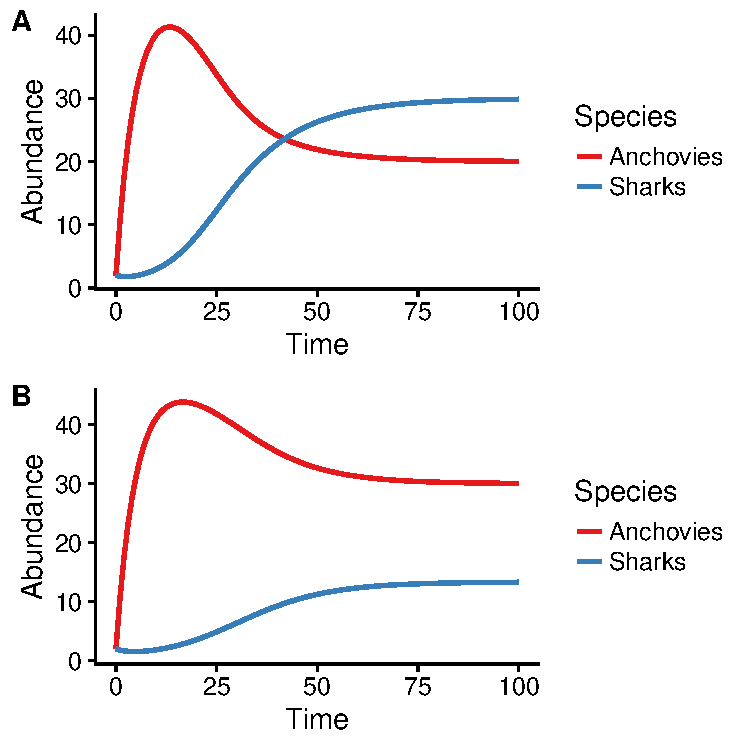
\includegraphics{AwesomeArticle_files/figure-latex/unnamed-chunk-8-1.pdf}
\caption{\label{fig:unnamed-chunk-8}\label{fig:timeseries}State variabel
dynamics through time for an ecosystem without fishing (A) and with
fishing (B).}
\end{figure}

\begin{table}[H]

\caption{\label{tab:unnamed-chunk-9}\label{tab:stable_eq}Stable equilibrium values for Sharks and Anchovies under fishing and no fishing conditions}
\centering
\begin{tabular}[t]{l|r|r}
\hline
Species & Fishing & No Fishing\\
\hline
Anchovies & 30.05 & 20.05\\
\hline
Sharks & 13.29 & 29.88\\
\hline
\end{tabular}
\end{table}

\section{Discusion and Conclusion}\label{discusion-and-conclusion}

Our results are not novel, because they had been shown before
\citep{szuwalski_2017}.

\clearpage

\bibliographystyle{frontiersinSCNS_ENG_HUMS}\bibliography{references}



\end{document}
